\documentclass[conference,compsoc]{IEEEtran}

\usepackage{cite}
\usepackage{amsmath,amssymb}
\usepackage{graphicx}
\usepackage{textcomp}
\usepackage{xcolor}
\usepackage{booktabs}
\usepackage{url}
\usepackage{microtype}
\usepackage{gensymb}

\graphicspath{{figures/}}
\newcommand{\degc}{\,\textdegree C}
\newcommand{\pp}{\,pp}
% expandable \input so generated table rows may start with \multicolumn
\makeatletter\newcommand{\tabinput}[1]{\@@input #1 }\makeatother

\begin{document}

\title{Thermal-Headroom Routing for Efficient Robot Perception in Extreme Heat}

\author{
\IEEEauthorblockN{Sparsh Roy\IEEEauthorrefmark{1}\IEEEauthorrefmark{2}\IEEEauthorrefmark{3},
Arhaan Shah\IEEEauthorrefmark{4},
Kevin Zhou\IEEEauthorrefmark{2},
\underline{\hspace{2.2cm}}\IEEEauthorrefmark{4},
\underline{\hspace{2.2cm}}\IEEEauthorrefmark{4},
\underline{\hspace{2.2cm}}\IEEEauthorrefmark{4}}
\IEEEauthorblockA{\IEEEauthorrefmark{1}Massachusetts Institute of Technology, Cambridge, MA, USA}
\IEEEauthorblockA{\IEEEauthorrefmark{2}Hopewell Valley Central High School, Pennington, NJ, USA}
\IEEEauthorblockA{\IEEEauthorrefmark{4}Paradise Valley High School, Phoenix, AZ, USA}
\IEEEauthorblockA{\IEEEauthorrefmark{3}Corresponding author: sparshr@mit.edu}
}

\maketitle

% ---------------------------------------------------------------
\begin{abstract}
A robot working in a Phoenix summer runs its detector on a small
embedded processor that heats itself. Once that processor hits its
thermal limit, the frequency governor throttles it and every detector
configuration gets slower at the same time. Adaptive inference routers,
which pick a model size and input resolution for each frame, usually
treat this slowdown as outside interference. In hot weather the router
causes it. We model the effect with a lumped RC thermal model wired in
closed loop to a deadline-constrained router over four YOLO11
configurations. We also propose Thermal-Headroom Routing (THR), which
forecasts the processor temperature in closed form before committing
to a configuration and skips any configuration that would push the chip
past its throttle threshold. We tested it on seven real traces with
camera degradation (off-road driving, rain, snow, fog, night, and lens
soiling), eight ambient temperatures, and five seeds. At 45\degc{} and
55\degc{} THR never throttled. A router driven only by latency belief
spent 11 to 38\% of each mission throttled. THR also lowered the
deadline-miss rate by 3.9 to 7.4 percentage points and energy per
on-time frame by 11 to 13\%, and it costs about 7\,$\mu$s per frame. At
35\degc{} and below it makes the same decisions as the baseline. A
control that gets the same share of heavy-model frames, but no
temperature reading, reaches the same miss rate. The miss-rate gain
therefore comes from the amount of heavy inference the router allows.
What the thermal forecast adds is a way to find that amount online, at
any ambient temperature, while keeping throttling at zero. Code and
outputs are public.%
\footnote{\url{https://github.com/ImSpxrsh/thermal-headroom-routing}}
\end{abstract}

\begin{IEEEkeywords}
efficient inference, adaptive model selection, thermal throttling,
edge AI, robot perception, extreme environments
\end{IEEEkeywords}

% ---------------------------------------------------------------
\section{Introduction}

Consider a Jetson-class module in a sealed enclosure on a robot in the
Sonoran Desert. The air is at 45\degc. If the perception stack runs its
largest detector on every frame, the chip reaches its throttle limit in
about a minute. The governor then down-clocks it, and the small models
slow down along with the large one until the chip cools
\cite{bhat2019power}. In our simulations a policy that always runs the
large model goes blind for 12.5\,s at a stretch at 45\degc, and for
91\,s at 55\degc{} (we count a blackout as a run of consecutive
deadline misses).

Adaptive inference is the usual answer to a tight latency budget.
Early-exit networks and routers choose cheaper computation per input or
per frame \cite{teerapittayanon2016branchynet,laskaridis2021adaptive,wang2021notallimages},
and some also watch current compute load. All of them react to latency
after it has risen. In heat that reaction comes late, because the
slowdown was set up by earlier choices and lasts for tens of seconds
once it starts. Thermal-aware scheduling for multiprocessors has dealt
with this kind of delayed feedback for years
\cite{coskun2007temperature,skadron2003hotspot}, and planetary rovers
plan compute around thermal and power limits
\cite{verma2023perseverance}. Per-frame model selection has not used
those ideas. Belief-space perception routing \cite{roy2026beliefspace},
which this work extends, tracks camera-fault and compute-contention
beliefs together but leaves thermal effects out of its contention model.

Our contributions:
(i) a closed-loop model of thermal contention for adaptive inference,
in which the router's configuration choice sets the power input to an
RC thermal node with a hysteretic throttle (\S\ref{sec:model});
(ii) THR, a closed-form rule that keeps the forecast temperature under
the throttle limit at about 7\,$\mu$s per frame and works alongside
fault-aware routing \cite{roy2026beliefspace} (\S\ref{sec:thr});
(iii) an evaluation on seven real degraded-camera traces over eight
ambient temperatures, with a cool-weather negative control and a
matched-budget control in the spirit of the matched-input controls in
\cite{zhou2026matchedinput}, which tells apart the effect of how much
heavy inference runs from the effect of when it runs
(\S\ref{sec:results}); and
(iv) power, energy and accuracy accounting for every policy, plus a
test of THR with a wrong thermal model.

% ---------------------------------------------------------------
\section{Related Work}

\textit{Adaptive and efficient inference.} Early-exit networks
\cite{teerapittayanon2016branchynet,laskaridis2021adaptive}, dynamic
transformers \cite{wang2021notallimages} and early exiting for driving
\cite{adee2025,navee2025,temporalpatience2023} vary computation with
the input. Modality gating \cite{dynmm,mees2016choosing,pramr2025}
decides which sensors to process at all. These methods treat the
compute budget as fixed or as something they observe. None of them
models the budget as a state their own decisions change.

\textit{Sensor- and compute-aware routing.} Belief-space perception
routing \cite{roy2026beliefspace} tracks blur, illumination and
occlusion faults per camera channel with switching HMMs, keeps a
latency-based contention belief, and fuses the two with a noisy-OR
term. When faults and contention were made to co-occur, that fusion cut
deadline misses by 1.1 to 9.4 percentage points. Its contention signal
comes from outside the router and has two states. We reuse its fault
beliefs, frontier and traces and add a thermal plant that the router
drives.

\textit{Thermal management.} HotSpot-style RC models
\cite{skadron2003hotspot} and temperature-aware MPSoC scheduling
\cite{coskun2007temperature} predict hot spots and schedule around
them. Measurements on commercial phone SoCs show throttling dominating
sustained performance \cite{bhat2019power}. We apply the same
forecasting idea to per-frame model selection, where the thing being
chosen is a point on the accuracy-latency curve.

\textit{Datasets.} The traces come from TartanDrive off-road driving
\cite{triest2022tartandrive,sivaprakasam2024tartandrive2}, RADIATE
adverse weather \cite{sheeny2021radiate} and WoodScape fisheye soiling
\cite{yogamani2019woodscape}.

% ---------------------------------------------------------------
\section{System Model}
\label{sec:model}

\textit{Frontier and deadline.} There are four configurations, from most
to least expensive: C1 is YOLO11x at 1280\,px, C2 is YOLO11x at 640, C3
is YOLO11n at 1280 and C4 is YOLO11n at 640. Their per-frame latencies
were profiled under normal and contended compute in
\cite{roy2026beliefspace}. The deadline $D$ is C1's median latency
under normal compute, between 211 and 341\,ms depending on the trace.
C1 therefore meets $D$ about half the time on a cool chip and almost
never on a slowed one. C2, C3 and C4 always meet it. Accuracy is the
IoU-matched F1 agreement between a configuration's detections and C1's
on the same frame. The earlier study found that this pseudo-ground
truth ranks configurations differently from real annotations
\cite{roy2026beliefspace}, so we treat every accuracy number here as an
internal consistency check. Deadline-miss, throttling and energy
results do not depend on it.

\textit{Thermal plant.} We model the SoC as one thermal node with time
constant $\tau$ and junction-to-ambient resistance $R_{\mathrm{th}}$:
\begin{equation}
T_{t+1} = T_t + \tfrac{\Delta t}{\tau}\big(T_{\mathrm{amb}} + R_{\mathrm{th}}\,P_t - T_t\big).
\label{eq:rc}
\end{equation}
Power depends on the configuration $c_t$ served at frame $t$:
$P_t = s_t\,[P_{\mathrm{idle}} + (P_{\max}-P_{\mathrm{idle}})\,u(c_t)]$.
Here $u(c)=\min(1,\tilde{\ell}_c/D)$ is the configuration's median
normal-compute latency as a fraction of the deadline, and $s_t$ is 0.6
while throttled and 1 otherwise. The governor starts throttling at
$T\ge T_{\mathrm{hi}}$ and stops at $T\le T_{\mathrm{lo}}$. While it
throttles, every configuration's latency is drawn from its profiled
contended distribution, whose p95 is about $2.5\times$ the normal one.
Table~\ref{tab:params} lists the parameters. They are typical of a
Jetson Orin module and were chosen before any run, but we did not
measure them. Running C1 nonstop settles at $T_{\mathrm{amb}}+50$\degc,
so throttling starts once the air is above 40\degc. The repository
includes a Jetson harness that logs \texttt{tegrastats} temperature and
power, which can supply measured values.

\begin{table}[t]
\caption{Thermal-plant parameters (typical values, fixed before any run).}
\label{tab:params}
\centering\footnotesize
\begin{tabular}{@{}lc@{\hspace{10pt}}lc@{}}
\toprule
$\Delta t$ (frame) & 0.1\,s & $P_{\mathrm{idle}}$ / $P_{\max}$ & 5 / 25\,W \\
$\tau$ & 30\,s & $T_{\mathrm{hi}}$ / $T_{\mathrm{lo}}$ & 90 / 85\degc \\
$R_{\mathrm{th}}$ & 2.0\,\textdegree C/W & throttled power & $0.6\times$ \\
\bottomrule
\end{tabular}
\end{table}

\textit{Closed loop.} In \cite{roy2026beliefspace} contention followed
a fixed schedule, so every policy could be scored against the same
pre-drawn timeline. Here, whether the chip is throttled at frame $t$
depends on what the router chose before $t$, so each policy has to run
in closed loop with the plant. For a given seed, all policies see the
same pre-drawn latency samples (normal and contended) and the same
sensor noise.

% ---------------------------------------------------------------
\section{Thermal-Headroom Routing}
\label{sec:thr}

All policies use the objective from \cite{roy2026beliefspace}. They
predict a compute state, keep the configurations whose median latency
in that state meets $D$, and serve the one with the highest expected
accuracy given the camera-fault belief $b_f$. A 10-frame dwell keeps
them from switching back and forth. They differ only in the inputs
they use.

\textit{Online compute belief.} In closed loop the router only learns
the latency of the configuration it served, and only one frame later.
We run a two-state forward filter (stay probabilities 0.95 and 0.90) on
one binary observation: whether the last latency exceeded $1.5\times$
that configuration's normal median. The filter output is $b_c$.

\textit{THR.} Let $\hat T$ be the on-die temperature reading (we add
Gaussian noise with $\sigma=1$\degc). If the router held configuration
$c$ for $H$ frames, Eq.~\eqref{eq:rc} gives the temperature in closed
form:
\begin{equation}
\hat T_{H}(c) = T_{\infty}(c) + \big(\hat T - T_{\infty}(c)\big)\big(1-\tfrac{\Delta t}{\tau}\big)^{H},
\label{eq:forecast}
\end{equation}
with $T_{\infty}(c)=T_{\mathrm{amb}}+R_{\mathrm{th}}P(c)$. THR drops $c$
from consideration when $\hat T_H(c) \ge T_{\mathrm{hi}}-m$, using
$H=50$ frames and a margin $m=2$\degc. C4 is always allowed, so some
configuration is always available. Feasibility and accuracy selection
then run as usual. Each frame costs four evaluations of
Eq.~\eqref{eq:forecast}. With the belief update and selection included,
we measured 7.3\,$\mu$s per frame in Python on one Apple M5 core, under
0.004\% of one C1 inference.

\textit{Joint + THR.} Camera faults sometimes come with extra compute
load, for example when a degraded camera makes localization work
harder. For that case THR can be combined with the noisy-OR coupling
of \cite{roy2026beliefspace}, $p_{\mathrm{cont}} = 1-(1-b_c)(1-\kappa b_f)$,
where $\kappa$ is fit on separate calibration draws.

\textit{Baselines.} Static C1 and Static C4 always serve one
configuration. Reactive looks at latency only and ignores the camera.
Belief is the decoupled router of \cite{roy2026beliefspace} using our
online $b_c$ and no temperature input. Joint adds the fault-coupling
term to Belief. Matched budget is Belief with a running cap on the
share of frames that use C1, set to the share THR used for the same
seed and ambient temperature. It has the same heavy-model budget as THR
and no temperature reading, which lets us check whether THR helps by
choosing good moments for C1 or simply by using C1 less.

% ---------------------------------------------------------------
\section{Experimental Setup}

\textit{Traces.} We use seven real traces with the frontiers and fault
labels profiled in \cite{roy2026beliefspace}. Two come from
TartanDrive: the full trajectory, which has no camera faults and serves
as a negative control, and a 309-frame stretch of rough terrain. Four
come from RADIATE (rain, snow, fog, night). The last is WoodScape
fisheye video with real soiling masks. We repeat each trace to fill a
1200-frame mission (2 minutes at 10\,Hz) so the chip has time to reach
thermal steady state.

\textit{Experiments.} E1 re-scores the original fault-coupled contention
schedule of \cite{roy2026beliefspace} for bursts of consecutive misses.
E2 has thermal contention only, at ambient temperatures of 20 to
55\degc{} in steps of 5. E3 adds the fault-coupled schedule on top of
thermal throttling. In E4, THR is given a wrong $R_{\mathrm{th}}$ or
$\tau$ while the plant keeps the true values.

\textit{Protocol.} We follow the validation-locked protocol of
\cite{zhou2026matchedinput}. Every tunable (plant parameters, $H$, $m$,
dwell, the 1.5$\times$ slow threshold) was set in code before the first
evaluation run, and none was changed after seeing results. Each result
file records \texttt{eval\_labels\_used\_for\_selection: false}. All
comparisons use five seeds, which change the latency draws, the camera
measurement noise and the temperature-sensor noise on the same real
frames. We report 95\% $t$-intervals on paired per-seed differences
and mark with $^\ast$ any interval that excludes zero.

% ---------------------------------------------------------------
\section{Results}
\label{sec:results}

\begin{figure*}[t]
\centering
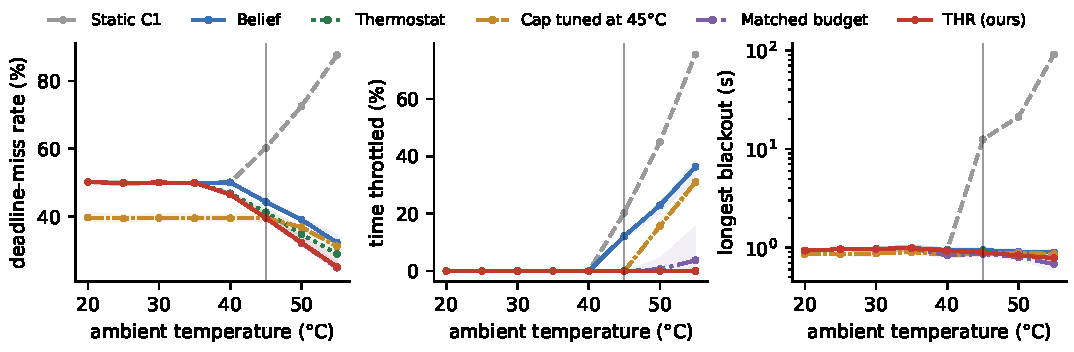
\includegraphics[width=\textwidth]{fig_heat_sweep.pdf}
\caption{Ambient sweep (E2). Lines are the mean over seven traces and
bands span the lowest and highest trace. Left: deadline-miss rate.
Middle: share of the mission spent throttled. Right: longest blackout
in seconds, log scale. THR (red) never throttles. Matched budget
(purple) has the same miss rate as THR but still throttles at 50 and
55\degc.}
\label{fig:sweep}
\end{figure*}

\subsection{Cool air}
From 20 to 35\degc{} no policy ever brings the chip to $T_{\mathrm{hi}}$.
THR, Belief, Reactive and Matched budget make the same choice on every
frame, and their miss rates differ by exactly 0.0 percentage points on
all seven traces (Fig.~\ref{fig:sweep}). THR only acts differently when
its forecast says the chip will cross the threshold. At 40\degc{} it
starts holding C1 back a little early: C1 serves about 93\% of frames
and pseudo-GT agreement stays between 0.97 and 1.00.

\subsection{Hot air}
Table~\ref{tab:eff} lists miss rate, throttling, blackout length,
power, energy and accuracy for each policy. Static C1 does badly. At
45\degc{} it is throttled 20\% of the time and has a 12.5\,s blackout
on every trace. At 55\degc{} it is throttled 76\% of the time, its
longest blackout is 91\,s, and it misses 88\% of deadlines.

Belief and Reactive keep the longest blackout near 1\,s, but they are
still throttled for 11 to 13\% of the mission at 45\degc{} and 32 to
39\% at 55\degc. Fig.~\ref{fig:trace} shows why. They respond to the
slowdown after the governor has already stepped in.

THR was never throttled on any trace, seed or temperature. Compared
with Belief it lowers the miss rate by 3.9 to 5.5 percentage points at
45\degc{} and by 6.5 to 7.4 at 55\degc, and every one of those
fourteen differences is significant (Table~\ref{tab:heat}). Energy per
on-time frame falls by 11\% at 45\degc{} (3.61 against 4.08\,J) and by
13\% at 55\degc{} (2.30 against 2.65\,J). THR pays for this with
accuracy, since it serves C1 less often: mean pseudo-GT agreement at
45\degc{} goes from 0.975 to 0.949. On-time utility, which scores a
frame by its accuracy if it is on time and zero otherwise, still rises
significantly on rain, snow, fog and night at 45\degc{} (by 2.1 to 4.4
points) and does not change on the other three traces. Static C4 beats
every policy on timing and energy, with agreement of only 0.695. THR
sits between the two static policies on the accuracy-timeliness
trade-off.

\begin{table}[t]
\caption{Efficiency, quality and cost in E2, averaged over 7 traces.
Miss and Thr.\ (throttled) in \%. Blackout is the longest run of
consecutive misses in seconds. $P$ is mean SoC power (W) and
$E_{\mathrm{ot}}$ is energy per on-time frame (J). Acc.\ is pseudo-GT
agreement (internal consistency only).}
\label{tab:eff}
\centering\footnotesize
\setlength{\tabcolsep}{3.2pt}
\begin{tabular}{@{}lcccccc@{}}
\toprule
Policy & Miss & Thr. & Blackout & $P$ & $E_{\mathrm{ot}}$ & Acc. \\
\midrule
\tabinput{tables/tab_efficiency.tex}
\bottomrule
\end{tabular}
\end{table}

\begin{figure}[t]
\centering
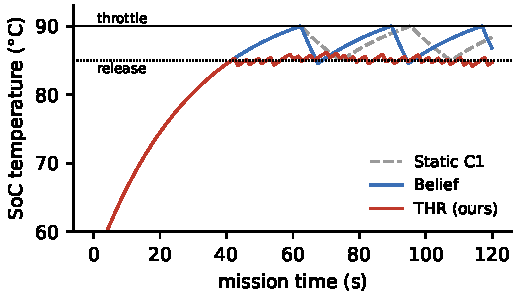
\includegraphics[width=\columnwidth]{fig_heat_trace.pdf}
\caption{SoC temperature during one 2-minute mission at 45\degc{} (fog
trace, seed 0). Static C1 and Belief go through repeated throttle
cycles. THR alternates C1 and C2 and stays just below the release
threshold.}
\label{fig:trace}
\end{figure}

\begin{table*}[t]
\caption{Heat regime (E2) per trace. Blackout C1 is Static C1's longest
run of consecutive misses (s). Thr.\ is the \% of the mission spent
throttled. $\Delta$ is the reduction in deadline-miss rate relative to
Belief, in percentage points (positive means fewer misses). THR$-$MB
compares THR with the matched-budget control. $^\ast$: the 95\% CI over
5 seeds excludes zero.}
\label{tab:heat}
\centering\footnotesize
\setlength{\tabcolsep}{3pt}
\resizebox{\textwidth}{!}{%
\begin{tabular}{@{}l cccccc c cccccc@{}}
\toprule
& \multicolumn{6}{c}{Ambient 45\degc} && \multicolumn{6}{c}{Ambient 55\degc} \\
\cmidrule{2-7}\cmidrule{9-14}
Trace & Blackout C1 & Thr.\ Belief & Thr.\ THR & $\Delta$ THR & $\Delta$ MB & THR$-$MB &&
Blackout C1 & Thr.\ Belief & Thr.\ THR & $\Delta$ THR & $\Delta$ MB & THR$-$MB \\
\midrule
\tabinput{tables/tab_heat_wide.tex}
\bottomrule
\end{tabular}}
\end{table*}

\subsection{Matched budget}
The matched-budget control uses C1 for the same share of frames as THR,
but it picks those frames without knowing the temperature. Its miss
rate is statistically indistinguishable from THR's on every trace at
both temperatures. The gap is never more than 1.0 percentage point and
no interval excludes zero (Table~\ref{tab:heat}). So most of THR's
deadline gain comes from how much C1 it runs. Forecasting the right
moments adds little on top. Part of the reason is the deadline rule.
$D$ is C1's median latency, so C1 misses about half its frames even on
a cool chip, and any policy that uses C1 less will miss less.

The two policies do differ on throttling. At 55\degc{} the matched
budget is still throttled on rain (4.5\% of the mission), fog (5.8\%)
and soiling (15.6\%), and those paired differences are significant.
THR is never throttled. The control also needed THR to tell it the
budget in the first place. The right C1 share falls from about 0.93 at
40\degc{} to between 0.48 and 0.56 at 55\degc, so a fixed cap tuned at
one temperature would waste accuracy or throttle at another. For an
efficiency-minded deployment, the forecast in THR works as a cheap way
to estimate the heavy-model budget online. A duty cap that lands on
the same budget by other means should do equally well on misses.

\subsection{Heat combined with camera faults}
E3 adds fault-coupled contention on top of throttling
(Fig.~\ref{fig:compound}, Table~\ref{tab:compound}). The fault-coupling
term and THR respond to different problems. On the fault-free
trajectory the coupling term (Joint) gains exactly 0.0 points, and THR
gains 5.3 points at 45\degc{} and 8.6 at 55\degc. At 25\degc{} THR adds
nothing, and Joint\,+\,THR matches Joint exactly. At 45 and 55\degc,
Joint\,+\,THR beats Belief on all seven traces, by 5.3 to 13.0 points
and by 6.9 to 13.7 points, and it never falls below Joint alone. At
55\degc{} Joint by itself is no longer significant on snow and soiling,
while Joint\,+\,THR is (9.0 and 6.9 points).

\begin{figure}[t]
\centering
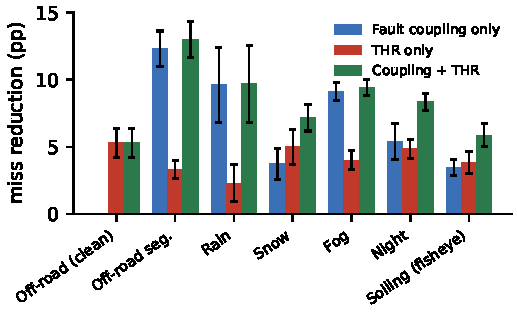
\includegraphics[width=\columnwidth]{fig_compound.pdf}
\caption{Heat plus fault-coupled contention at 45\degc{} (E3). Bars show
the reduction in deadline-miss rate relative to Belief, with 95\%
CIs. Joint\,+\,THR is best or tied on every trace.}
\label{fig:compound}
\end{figure}

\begin{table}[t]
\caption{E3: reduction in miss rate relative to Belief (pp). J is
Joint (fault coupling only); J+T is Joint\,+\,THR.}
\label{tab:compound}
\centering\footnotesize
\setlength{\tabcolsep}{3pt}
\begin{tabular}{@{}lcccccc@{}}
\toprule
& \multicolumn{2}{c}{25\degc} & \multicolumn{2}{c}{45\degc} & \multicolumn{2}{c}{55\degc} \\
\cmidrule(lr){2-3}\cmidrule(lr){4-5}\cmidrule(l){6-7}
Trace & J & J+T & J & J+T & J & J+T \\
\midrule
\tabinput{tables/tab_compound.tex}
\bottomrule
\end{tabular}
\end{table}

\subsection{Wrong thermal model}
A real deployment would have to estimate $R_{\mathrm{th}}$ and $\tau$.
In E4 (Table~\ref{tab:misspec}) we change the model THR believes in
while leaving the plant alone, at 45\degc. Because THR forecasts from
the measured temperature, no error we tried brought throttling back on
any trace. The errors change how cautious THR is. If it thinks
$R_{\mathrm{th}}$ is 30\% lower than it is, the miss-rate gain shrinks
to 0.6 to 2.3 points (significant on 5 of 7 traces) and more accuracy
is kept. Overestimating $R_{\mathrm{th}}$ or underestimating $\tau$
gives larger miss reductions and lower accuracy. A rough model is
enough to avoid throttling, and the value of $R_{\mathrm{th}}$ mostly
decides where THR lands between accuracy and timeliness.

\begin{table}[t]
\caption{THR with a wrong thermal model at 45\degc{} (E4): range of the
miss-rate reduction relative to Belief over 7 traces, number of traces
with a significant reduction, accuracy range, and the largest throttled
share.}
\label{tab:misspec}
\centering\footnotesize
\setlength{\tabcolsep}{3.5pt}
\begin{tabular}{@{}lcccc@{}}
\toprule
THR's model & $\Delta$ miss (pp) & Sig. & Acc. & Max thr.\ (\%) \\
\midrule
\tabinput{tables/tab_misspec.tex}
\bottomrule
\end{tabular}
\end{table}

\subsection{Bursts of misses under fault-coupled contention}
A field robot cares about how long it goes without a usable detection,
and the average miss rate hides that. We re-scored the original
fault-coupled schedule of \cite{roy2026beliefspace} (E1,
Table~\ref{tab:bursts}). Fault coupling lowers the share of frames that
fall inside bursts of three or more misses (0.3\,s) on 4 of 7 traces:
by 2.7 points on the off-road stretch, 6.3 on fog, 3.3 on night and 1.0
on soiling. It is exactly zero on the clean trajectory. On no trace
does it significantly shorten the longest blackout. Coupling makes
bursts less frequent, but the worst case stays about where it was.

\begin{table}[t]
\caption{Bursts under fault-coupled contention (E1). Burst share is the
\% of frames inside runs of at least 3 misses. Max run is in frames.}
\label{tab:bursts}
\centering\footnotesize
\setlength{\tabcolsep}{3.5pt}
\begin{tabular}{@{}lccccc@{}}
\toprule
& \multicolumn{2}{c}{Burst share (\%)} & & \multicolumn{2}{c}{Max run} \\
\cmidrule(lr){2-3}\cmidrule(l){5-6}
Trace & Belief & Joint & $\Delta$ (pp) & Belief & Joint \\
\midrule
\tabinput{tables/tab_bursts.tex}
\bottomrule
\end{tabular}
\end{table}

% ---------------------------------------------------------------
\section{Discussion and Limitations}

In a closed-loop simulation built on real camera traces and real
profiled latencies, a closed-form thermal forecast kept the chip out of
throttling at a cost of microseconds per frame. It lowered deadline
misses and energy per on-time frame in hot air, changed nothing below
40\degc, and worked alongside fault-aware routing. The matched-budget result limits what we can claim. A duty cap
with no temperature input does as well on misses once it has the same
budget, so the finding is about budgeting heavy inference. We have not
shown that THR's choice of when to run C1 matters on its own.

The simulation has clear gaps. The plant is one RC node with typical
parameters that we did not measure. Throttling reuses the profiled
contended latency distribution instead of real DVFS states. Latencies
were measured on an Apple M5 GPU, not an embedded module. Traces are
repeated to reach mission length. Accuracy is agreement with the
largest model, which tracks real annotations poorly
\cite{roy2026beliefspace}, so accuracy and utility numbers only show
internal consistency. Seeds change noise on fixed frames and do not
stand in for independent missions.

Next, we plan to measure $R_{\mathrm{th}}$, $\tau$ and throttle
behaviour on a Jetson Orin inside an environmental chamber from 25 to
55\degc{} using the \texttt{tegrastats} harness, and to score the
routers against real annotations. We would also like to learn the duty
budget directly from temperature logs, which would remove the need for
an RC model.

% ---------------------------------------------------------------
\section{Conclusion}

On a hot robot, choosing a heavy model now can cause throttling a
minute later. THR gives the router a closed-form temperature forecast
that costs microseconds per frame. Across seven real camera traces at
45 and 55\degc{} the chip never throttled under THR. Deadline misses
dropped by 3.9 to 7.4 percentage points and energy per on-time frame by
11 to 13\%, while cool-weather behaviour stayed the same. The
matched-budget control shows that the share of heavy-model frames is
what drives the miss-rate gain. Teams building perception for hot
hardware should estimate that share online from temperature instead of
fixing it ahead of time.

\section*{Acknowledgment}
This work builds on the code and traces of belief-space perception
routing \cite{roy2026beliefspace}. We thank Vihan Aggarwal and Davin
Yin for that work.

\bibliographystyle{IEEEtran}
\bibliography{references}

\end{document}
